\documentclass[a4paper,12pt]{article}

\textwidth 17cm \textheight 25cm \evensidemargin 0cm
\oddsidemargin 0cm \topmargin -2cm
\parindent 0pt
%\parskip \bigskipamount

\usepackage{graphicx}
\usepackage[dutch]{babel}
\usepackage{amssymb,amsthm,amsmath}
%\usepackage{dot2texi}
\usepackage[utf8]{inputenc}
\usepackage{nopageno}
\usepackage{pdfpages}
\usepackage{enumerate}
\usepackage{caption}
\usepackage{wrapfig}
\usepackage{pgf,tikz,pgfplots}
\pgfplotsset{compat=1.15}
\usepackage{color}
\usetikzlibrary{arrows}
\usetikzlibrary{patterns}
\usepackage{fancyhdr}
\pagestyle{fancy}
\usepackage[version=3]{mhchem}
\usepackage{multicol}
\usepackage{fix-cm}
\usepackage{setspace}
\usepackage{mhchem}
\usepackage{xhfill}
\usepackage{parskip}
\usepackage{cancel}
\usepackage{mdframed}
\usepackage{url}
\usepackage{mathtools}
\usepackage{changepage}

\newcommand{\todo}[1]{{\color{red} TODO: #1}}

\newcommand{\degree}{\ensuremath{^\circ}}
\newcommand\rad{\qopname\relax o{\mathrm{rad}}}

\newcommand\ggd{\qopname\relax o{\mathrm{ggd}}}

\pgfmathdeclarefunction{gauss}{2}{%
  \pgfmathparse{1/(#2*sqrt(2*pi))*exp(-((x-#1)^2)/(2*#2^2))}%
}

\def\LRA{\Leftrightarrow}

\newcommand{\zrmbox}{\framebox{\phantom{EXE}}\phantom{X}}
\newcommand{\zrm}[1]{\framebox{#1}}

% environment oefening:
% houdt een teller bij die de oefeningen nummert, probeert ook de oefening op één pagina te houden
\newcounter{noefening}
\setcounter{noefening}{0}
\newenvironment{oefening}
{
  \stepcounter{noefening}
  \pagebreak[0]
  \begin{minipage}{\textwidth}
  \vspace*{0.7cm}{\large\bf Oefening \arabic{noefening}}
}{%
  \end{minipage}
}

\usepackage{calc}

% vraag
\reversemarginpar
\newcounter{punten}
\setcounter{punten}{0}
\newcounter{nvraag}
\setcounter{nvraag}{1}
\newlength{\puntwidth}
\newlength{\boxwidth}
\newcommand{\vraag}[1]{
\settowidth{\puntwidth}{\Large{#1}}
\setlength{\boxwidth}{1.5cm}
\addtolength{\boxwidth}{-\puntwidth}
{\large\bf Vraag \arabic{nvraag} \addtocounter{nvraag}{1}}\vspace*{-0.5cm}
{\marginpar{\color{lightgray}\fbox{\parbox{1.5cm}{\vspace*{1cm}\hspace*{\boxwidth}{\Large{#1}}}}}
\vspace*{0.5cm}}
\addtocounter{punten}{#1}}

% arulefill
\def\arulefill{\leavevmode{\xrfill[-5pt]{0.3pt}[lightgray]\endgraf}\vspace*{0.2cm}}

% \arules{n}
\newcommand{\arules}[1]{
\color{lightgray}
%\vspace*{0.05cm}
\foreach \n in {1,...,#1}{
  \vspace*{0.75cm}
  \hrule height 0.3pt\hfill
}\color{black}\vspace*{0.2cm}}

% \arule{x}
\newcommand{\arule}[1]{
\color{lightgray}{\raisebox{-0.1cm}{\rule[-0.05cm]{#1}{0.3pt}}}\color{black}
}

% \abox{y}
\newcommand{\abox}[1]{
\fbox{
\begin{minipage}{\textwidth- 4\fboxsep}
\hspace*{\textwidth}\vspace{#1}
\end{minipage}
}
}

\newcommand{\ruitjes}[1]{
\definecolor{cqcqcq}{rgb}{0.85,0.85,0.85}
\hspace*{-2.5cm}
\begin{tikzpicture}[scale=1.04,line cap=round,line join=round,>=triangle 45,x=1.0cm,y=1.0cm]
\draw [color=cqcqcq, xstep=0.5cm, ystep=0.5cm] (0,-#1) grid (20.5,0);
\end{tikzpicture}
}


\newcommand{\assenstelsel}[5][1]{
\definecolor{cqcqcq}{rgb}{0.65,0.65,0.65}
\begin{tikzpicture}[line cap=round,line join=round,>=triangle 45,x=#1cm,y=#1cm]
\draw [color=cqcqcq,dash pattern=on 1pt off 1pt, xstep=1.0cm,ystep=1.0cm] (#2,#4) grid (#3,#5);
\draw[->,color=black] (#2,0) -- (#3,0);
%\draw[shift={(1,0)},color=black] (0pt,2pt) -- (0pt,-2pt) node[below] {\footnotesize $1$};
%\draw[color=black] (#3.25,0.07) node [anchor=south west] {$x$};
\draw[->,color=black] (0,#4) -- (0,#5);
%\draw[shift={(0,1)},color=black] (2pt,0pt) -- (-2pt,0pt) node[left] {\footnotesize $1$};
\draw[color=black] (0.09,#5.25) node [anchor=west] {\phantom{$y$}};
%\draw[color=black] (0pt,-10pt) node[right] {\footnotesize $0$};
\end{tikzpicture}
}

\newcommand{\getallenas}[3][1]{
\definecolor{cqcqcq}{rgb}{0.65,0.65,0.65}
\begin{tikzpicture}[scale=#1,line cap=round,line join=round,>=triangle 45,x=1.0cm,y=1.0cm]
\draw [color=cqcqcq,dash pattern=on 1pt off 1pt, xstep=1.0cm,ystep=1.0cm] (#2,-0.2) grid (#3,0.2);
\draw[->,color=black] (#2.25,0) -- (#3.5,0);
\draw[shift={(0,0)},color=black] (0pt,2pt) -- (0pt,-2pt) node[below] {\footnotesize $0$};
\draw[shift={(1,0)},color=black] (0pt,2pt) -- (0pt,-2pt) node[below] {\footnotesize $1$};
\draw[color=black] (#3.25,0.07) node [anchor=south west] {$\mathbb{R}$};
\end{tikzpicture}
}

\newcommand{\visgraad}[1]{\begin{tabular}{p{0.5cm}|p{#1}}&\\\hline\\\end{tabular}}

\newcommand{\tekenschema}[2]{\begin{tabular}{p{0.5cm}|p{#1}}&\\\hline\\[#2]\end{tabular}}

% schema van Horner
\newcommand{\schemahorner}{
\begin{tabular}{p{0.5cm}|p{7cm}}
&\\[1.5cm]
\hline\\
\end{tabular}}

% geef tabular iets meer ruimte
\setlength{\tabcolsep}{14pt}
\renewcommand{\arraystretch}{1.5}

\newcommand{\toets}[3]{
\thispagestyle{plain}
\vspace*{-2.5cm}
\begin{tikzpicture}[remember picture, overlay]
    \node [shift={(15.25 cm,-1.6cm)}] {%
        \includegraphics[width=1.8cm]{/home/ppareit/kaa1415/logokaavelgem.png}%
    };%
\end{tikzpicture}

\begin{tabular}{|llc|c|}
\hline
\vspace*{-0.5cm}
&&&\\
Naam & \arule{4cm} & {\Large\bf KA AVELGEM} & \\
\vspace*{-0.75cm}
&&&\\
Klas & \arule{4cm} & {\Large\bf 20...-...-...} & \\
\hline
\vspace*{-0.75cm}
&&&\\
Toets & {\bf #2} & {\large\bf #1} & Beoordeling\\
\vspace*{-0.75cm}
&&&\\
Onderwerp & \multicolumn{2}{l|}{\bf #3} &\\
\hline
\end{tabular}
}

\newcommand{\oefeningen}[1]{

\fancyhead[LE, RO]{\vspace{0.5cm} #1}
%\thispagestyle{plain}

{\bf \Large \centering Oefeningen: #1}

}

\raggedbottom

\newcommand\vl{\qopname\relax o{\mathrm{vl}}}

\newcommand\dom{\qopname\relax o{\mathrm{dom}}}
\newcommand\ber{\qopname\relax o{\mathrm{ber}}}

\newcommand\mC{\qopname\relax o{\mathrm{mC}}}
\newcommand\uC{\qopname\relax o{\mathrm{{\mu}C}}}
\newcommand\C{\qopname\relax o{\mathrm{C}}}

\newcommand\W{\qopname\relax o{\mathrm{W}}}
\newcommand\kW{\qopname\relax o{\mathrm{kW}}}
\newcommand\kWh{\qopname\relax o{\mathrm{kWh}}}


\newcommand\V{\qopname\relax o{\mathrm{V}}}
\newcommand\ohm{\qopname\relax o{\mathrm{\Omega}}}
\newcommand\kohm{\qopname\relax o{\mathrm{k\Omega}}}


\newcommand\N{\qopname\relax o{\mathrm{N}}}

\newcommand\Nperkg{\qopname\relax o{\mathrm{N/kg}}}

\newcommand\Nperm{\qopname\relax o{\mathrm{N/m}}}

\newcommand\gpermol{\qopname\relax o{\mathrm{g/mol}}}


\newcommand\kgperm{\qopname\relax o{\mathrm{kg/m}}}
\newcommand\kgperdm{\qopname\relax o{\mathrm{kg/dm}}}
\newcommand\gpercm{\qopname\relax o{\mathrm{g/cm}}}
\newcommand\gperml{\qopname\relax o{\mathrm{g/ml}}}


\newcommand{\mA}{\;\mbox{mA}}
\newcommand{\A}{\;\mbox{A}}
\newcommand{\MA}{\;\mbox{MA}}

\newcommand{\us}{\;\mu\mbox{s}}
\newcommand\s{\qopname\relax o{\mathrm{s}}}

\newcommand\h{\qopname\relax o{\mathrm{h}}}

\newcommand{\kmperh}{\;\mbox{km/h}}
\newcommand{\mpers}{\;\mbox{m/s}}
\newcommand{\kmpermin}{\;\mbox{km/min}}
\newcommand{\kmpers}{\;\mbox{km/s}}

\newcommand{\mph}{\;\mbox{mph}}

\newcommand{\Hz}{\;\mbox{Hz}}

\newcommand\Gm{\qopname\relax o{\mathrm{Gm}}}
\newcommand\Mm{\qopname\relax o{\mathrm{Mm}}}
\newcommand\km{\qopname\relax o{\mathrm{km}}}
\newcommand\hm{\qopname\relax o{\mathrm{hm}}}
\newcommand\dam{\qopname\relax o{\mathrm{dam}}}
\newcommand\m{\qopname\relax o{\mathrm{m}}}
\newcommand\dm{\qopname\relax o{\mathrm{dm}}}
\newcommand\cm{\qopname\relax o{\mathrm{cm}}}
\newcommand\mm{\qopname\relax o{\mathrm{mm}}}
\newcommand\um{\qopname\relax o{\mathrm{{\mu}m}}}
\newcommand\nm{\qopname\relax o{\mathrm{nm}}}


\newcommand\Gg{\qopname\relax o{\mathrm{Gg}}}
\newcommand\Mg{\qopname\relax o{\mathrm{Mg}}}
\newcommand\kg{\qopname\relax o{\mathrm{kg}}}
\newcommand\hg{\qopname\relax o{\mathrm{hg}}}
\renewcommand\dag{\qopname\relax o{\mathrm{dag}}}
\newcommand\g{\qopname\relax o{\mathrm{g}}}
\newcommand\dg{\qopname\relax o{\mathrm{dg}}}
\newcommand\cg{\qopname\relax o{\mathrm{cg}}}
\newcommand\mg{\qopname\relax o{\mathrm{mg}}}
\newcommand\ug{\qopname\relax o{\mathrm{{\mu}g}}}
\renewcommand\ng{\qopname\relax o{\mathrm{ng}}}

\newcommand\ton{\qopname\relax o{\mathrm{ton}}}

\newcommand\Gl{\qopname\relax o{\mathrm{Gl}}}
\newcommand\Ml{\qopname\relax o{\mathrm{Ml}}}
\newcommand\kl{\qopname\relax o{\mathrm{kl}}}
\newcommand\hl{\qopname\relax o{\mathrm{hl}}}
\newcommand\dal{\qopname\relax o{\mathrm{dal}}}
\renewcommand\l{\qopname\relax o{\mathrm{l}}}
\newcommand\dl{\qopname\relax o{\mathrm{dl}}}
\newcommand\cl{\qopname\relax o{\mathrm{cl}}}
\newcommand\ml{\qopname\relax o{\mathrm{ml}}}
\newcommand\ul{\qopname\relax o{\mathrm{{\mu}l}}}
\newcommand\nl{\qopname\relax o{\mathrm{nl}}}

\newcommand\MJ{\qopname\relax o{\mathrm{MJ}}}
\newcommand\kJ{\qopname\relax o{\mathrm{kJ}}}
\newcommand\J{\qopname\relax o{\mathrm{J}}}

\newcommand\T{\qopname\relax o{\mathrm{T}}}
\newcommand\uT{\qopname\relax o{\mathrm{{\mu}T}}}

\newcommand\grC{\qopname\relax o{\mathrm{{\degree}C}}}

\newcommand\K{\qopname\relax o{\mathrm{K}}}
\newcommand\calperK{\qopname\relax o{\mathrm{cal/K}}}

\newcommand\hPa{\qopname\relax o{\mathrm{hPa}}}
\newcommand\Pa{\qopname\relax o{\mathrm{Pa}}}

\newcommand\dB{\qopname\relax o{\mathrm{dB}}}

\newcommand\Var{\qopname\relax o{\mathrm{Var}}}

\newcommand{\EE}[1]{\cdot 10^{#1}}

\onehalfspacing

%\setlength{\headsep}{0cm}

\newenvironment{exlist}[1] %
{ \begin{multicols}{#1}
  \begin{enumerate}[(a)]
    \setlength{\itemsep}{0.5em} }
{ \end{enumerate}
  \end{multicols} }




\usepackage{versions}
\includeversion{theorie}
%\excludeversion{theorie}

\begin{document}

\pagestyle{fancy}
\lhead{}
\rhead{Oefeningen Integraalrekening}

\begin{theorie}

\thispagestyle{empty}
\begin{center}
  \begin{mdframed}
  \centering
  \fontsize{40}{50}\selectfont Integraalrekening
  \end{mdframed}
  \vfill
  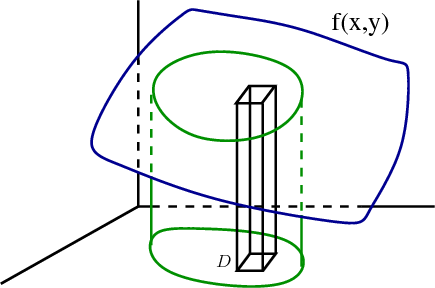
\includegraphics[width=.5\textwidth]{double_integral_volume_under_surface_box}
  \vfill
\end{center}

{
\small
\singlespacing
\subsection*{Doelstelling}
Je \hfill  {\scriptsize(LP 2006-059, LI 1.10)}
\begin{itemize}
  \item kan het begrip differentiaal en de meetkundige betekenis ervan
  \item kent het begrip bepaalde integraal
  \item kan het verband uitleggen tussen de bepaalde integraal van een functie en de oppervlakte van een gebied bepaald door de functie en de $x$-as
  \item kent het begrip primitieve functie
  \item kent de onderstaande eigenschappen:
  \begin{itemize}
    \item de stelling in verband met de optelbaarheid van de bepaalde integraal,
    \item de middelwaardenstelling,
    \item de hoofdstelling van de integraalrekening,
    \item de stelling in verband met de lineariteit van de bepaalde integraal,
    \item de stelling in verband met de bepaalde integraal en ongelijkheden
  \end{itemize}
  \item kan het verband illustreren tussen het berekenen van de bepaalde integraal van een functie en de primitieve van de gegeven functie
  \item kan bij het integreren van eenvoudige veeltermfuncties, rationale functies, irrationale functies, exponentiële functies, logaritmische functies en goniometrische functies gebruik maken van:
  \begin{itemize}
    \item de basisformules van de integraalrekening;
    \item de substitutiemethode;
    \item de methode van partiële integratie
  \end{itemize}
  \item kan vraagstukken/problemen oplossen (ook van buiten de wiskunde) die kunnen herleid worden tot het berekenen van een integraal
\end{itemize}
}

\pagestyle{empty}
\mbox{}
\newpage
\clearpage
\thispagestyle{empty}
%\mbox{}
{\small \tableofcontents}
\newpage
\clearpage
\pagenumbering{arabic}

\pagestyle{fancy}
\lhead{}
\rhead{Integraalrekening}

\end{theorie}

\onehalfspacing

\section{Differentiaal}

\begin{theorie}
\subsection{Differentiaal van een willekeurige functie}

In volgende figuur kennen we het verloop van de functie $f$ tot aan $x=a$. We willen een voorspelling doen over $f(b)$. Noem $\Delta x=b-a$. We willen dus weten wat $\Delta y=f(b)-f(a)$ is. We zijn tevreden met een benadering van $\Delta y$.

\begin{center}
\definecolor{wqwqwq}{rgb}{0.38,0.38,0.38}
\definecolor{uququq}{rgb}{0.25,0.25,0.25}
\begin{tikzpicture}[scale=1.3,line cap=round,line join=round,>=triangle 45,x=1.0cm,y=1.0cm]
\draw[->,color=black] (-3.3,0) -- (7.19,0);
\foreach \x in {-2,2,4,6}
\draw[shift={(\x,0)},color=black] (0pt,2pt) -- (0pt,-2pt);
\draw[->,color=black] (0,-1.41) -- (0,4.84);
\foreach \y in {,2,4}
\draw[shift={(0,\y)},color=black] (2pt,0pt) -- (-2pt,0pt);
\clip(-3.3,-1.41) rectangle (7.19,4.84);
\draw(2.93,6.98) -- (5.18,6.98);
\draw[line width=1.6pt, smooth,samples=100,domain=-3.302227053746148:7.191102772295233] plot(\x,{1/500*((\x)+2.5)*((\x)-6.5)*((\x)+0.5)*((\x)-3.5)*((\x)-9.5)+3});
\draw(2.88,7.93) -- (5.14,7.93);
\draw [line width=1.2pt,dotted,color=wqwqwq,domain=-3.3:7.19] plot(\x,{(--0.95--0.46*\x)/1});
\draw (-2.78,3.55) node[anchor=north west] {f};
\draw (2,1.86)-- (4,1.86);
\draw (4,1.86)-- (4,3.4);
\draw (2.81,1.86) node[anchor=north west] {$\Delta x$};
\begin{scriptsize}
\fill [color=black] (4.05,6.98) circle (1.5pt);
\draw[color=black] (4.19,7.39) node {$b = 4$};
\fill [color=black] (4.01,7.93) circle (1.5pt);
\draw[color=black] (4.14,8.34) node {$a = 2$};
\fill [color=uququq] (4,1.86) circle (1.5pt);
\draw[color=uququq] (4.23,1.64) node {$C$};
\draw[color=wqwqwq] (-2.67,-0.55) node {$t$};
\fill [color=uququq] (2,1.86) circle (1.5pt);
\draw[color=uququq] (1.68,2.31) node {$A$};
\fill [color=uququq] (4,3.4) circle (1.5pt);
\draw[color=uququq] (3.92,3.87) node {$B$};
\fill [color=uququq] (4,2.77) circle (1.5pt);
\draw[color=uququq] (4.33,2.65) node {$D$};
\fill [color=uququq] (2,0) circle (1.5pt);
\draw[color=uququq] (2.02,-0.35) node {a};
\fill [color=uququq] (4,0) circle (1.5pt);
\draw[color=uququq] (4.03,-0.35) node {b};
\end{scriptsize}
\end{tikzpicture}
\end{center}

Voor de eenvoud noemen we $(a,f(a))=A$, $(b,f(b))=B$ en $(b,f(a))=C$. We zoeken dus de afstand $\Delta y=|BC|$. Teken nu de raaklijn $t$ van $f$ in $A$ en noem het snijpunt $BC \cap t=D$.Als $A$ en $B$ voldoende dicht bij elkaar liggen wordt $\Delta y$ benaderd door $|CD|$.

We berekenen nu de rico $m$ van $t$ op 2 manieren:
\begin{itemize}
  \item M.b.v. definitie rico waarbij $(x_1,y_1)$ en $(x_2, y_2)$ zelf te kiezen punten op $t$ zijn:
  $$m=\dfrac{y_2-y_1}{x_2-x_1}=\dfrac{y_D-y_A}{x_D-x_A}=\dfrac{y_D-y_C}{b-a}=\dfrac{y_D-y_C}{\Delta x}$$
  \item M.b.v. afgeleid getal waarbij we omdat $t$ een rechte is zelf mogen kiezen waar:
  $$m = f'(a)$$
\end{itemize}

Onze rico elimineren we uit bovenstaande vergelijkingen:
\begin{align*}
     f'(a)     &= \dfrac{y_D-y_C}{\Delta x}\\
\LRA \qquad y_D - y_C &= f'(a)\cdot \Delta x\\
                      &= \mbox{differentiaal van $f$ in $a$}\\
                      &= \mbox{benadering voor $\Delta y$}\\
\end{align*}

We noteren deze benadering als $df(a)$. Merk op dat we uit de notatie de afstand $\Delta x$ laten verdwijnen. Dit omdat we in de toekomst $\Delta x$ oneindig klein zullen veronderstellen. Zodoende wordt de benadering exact! We krijgen dus volgende definitie.

\subsection{Definitie}
Voor een functie $f$ die afleidbaar is in $x$ en voor een $\Delta x$ die een toename is die oneindig klein wordt noemen we de differentiaal van $f$ in $x$ het product
$$df(x)=f'(x)\cdot\Delta x$$

\end{theorie}

\begin{oefening}
Bereken
\begin{multicols}{2}
\begin{enumerate}[(a)]
  \itemsep1em
  \item $\displaystyle d(x^4)$
  \item $\displaystyle d(\ln x)$
  \item $\displaystyle d(\sin x)$
  \item $\displaystyle d(x^3-2x)$
\end{enumerate}
\end{multicols}
\end{oefening}

\begin{theorie}

\subsection{Elimineren van $\Delta x$}

We berekenen de differentiaal van $f(x)=x$:
\begin{align*}
  df(x) &= f'(x)\Delta x\\
        &= x' \Delta x\\
        &= 1 \Delta x\\
        &= \Delta x\\
\end{align*}
Maar $df(x) = dx$ en dus $\Delta x = dx$. We mogen onze definitie dus aanpassen tot
$$df(x)=f'(x)\cdot dx$$

\end{theorie}

\begin{oefening}
Bereken
\begin{multicols}{2}
\begin{enumerate}[(a)]
  \itemsep1em
  \item $\displaystyle d\left(\dfrac{1}{x^2}\right)$
  \item $\displaystyle d\left(\log_2 x\right)$
  \item $\displaystyle d\left(\tan x\right)$
  \item $\displaystyle d\left(\frac{1}{3}x^3+\frac{1}{2}x^2+x+1\right)$
\end{enumerate}
\end{multicols}
\end{oefening}

\begin{theorie}

\subsection{Rekenregels voor het differentiëren}

\begin{mdframed}
\begin{multicols}{2}
  \begin{align*}
    dc &= 0\\
    dx^n &= nx^{n-1}dx\\
    d\sqrt{x}&=\dfrac{1}{2\sqrt{x}}dx\\
  \end{align*}
  \begin{align*}
    d(f+g) &= df + dg\\
    d(f\cdot g) &= df\cdot g + f\cdot dg\\
    d(c\cdot f) &= c\cdot f\\
    d\left(\dfrac{f}{g}\right) &=\dfrac{df\cdot g - f\cdot dg}{g^2}
  \end{align*}
  \begin{align*}
    de^x &= e^xdx\\
    da^x &= a^x\ln(a) dx\\
  \end{align*}
  \begin{align*}
    d\ln(x) &= \dfrac{1}{x}dx\\
    d\log_a(x) &= \dfrac{1}{x\cdot\ln a}dx\\
  \end{align*}
  \begin{align*}
    d\sin x &= \cos x \cdot dx\\
    d\cos x &= -\sin x \cdot dx\\
    d\tan x &= \dfrac{1}{\cos^2 x} \cdot dx\\
  \end{align*}
\end{multicols}
\end{mdframed}

Merk op dat we de kettingregel gratis krijgen! Zie volgende voorbeeld:

\begin{align*}
  d\sin\sqrt{x} &= \cos\sqrt{x} \cdot d\sqrt{x}\\
                &= \cos\sqrt{x} \cdot \dfrac{1}{2\sqrt{x}} \cdot dx\\
                &= \dfrac{\cos\sqrt{x}}{2\sqrt{x}} dx
\end{align*}

\end{theorie}

\begin{oefening}
Bepaal de differentiaal van de volgende functies
\begin{multicols}{2}
\begin{enumerate}[(a)]
  \itemsep.5em
  \item $\displaystyle f(x)=x^3+x$
  \item $\displaystyle f(x)=(x-2)(x+2)-x^2$
  \item $\displaystyle f(x)=5+3x^2+8x^4$
  \item $\displaystyle f(x)=\left(2x-4\right)^3$
  \item $\displaystyle f(x)=\left(x^2+x^4+x^6\right)^4$
  \item $\displaystyle f(x)=\sqrt{x^2+2x}$
  \item $\displaystyle f(x)=\sqrt[5]{6x^5+5x}$
  \item $\displaystyle f(x)=x^2\cdot\sqrt{x}$
  \item $\displaystyle f(x)=x^2\cdot\sqrt{x+1}$
  \item $\displaystyle f(x)=\dfrac{2x+1}{2x-1}$
  \item $\displaystyle f(x)=\dfrac{x^2-1}{x-1}$
  \item $\displaystyle f(x)=\dfrac{x^2-1}{x^2+1}$
  \item $\displaystyle f(x)=\dfrac{x^3+3x^2+3x+1}{x+1}$
  \item $\displaystyle f(x)=4^{x}$
  \item $\displaystyle f(x)=e^{-2x}$
  \item $\displaystyle f(x)=e^{\sqrt[3]{3x}}$
  \item $\displaystyle f(x)=\log_2 x$
  \item $\displaystyle f(x)=\log_2 (x^2-9)$
  \item $\displaystyle f(x)=x\cdot \ln x$
  \item $\displaystyle f(x)=x\cdot \ln x^2$
  \item $\displaystyle f(x)=\dfrac{1}{\ln 10}\cdot 10^{x^2}$
  \item $\displaystyle f(x)=x\sin x + \cos x$
\end{enumerate}
\end{multicols}
\end{oefening}

\begin{theorie}

\subsection{Toepassing}

Benader de waarde van $\log_2 5$, veronderstel dat je rekentoestel geen logaritmen kan uitrekenen.

\begin{center}
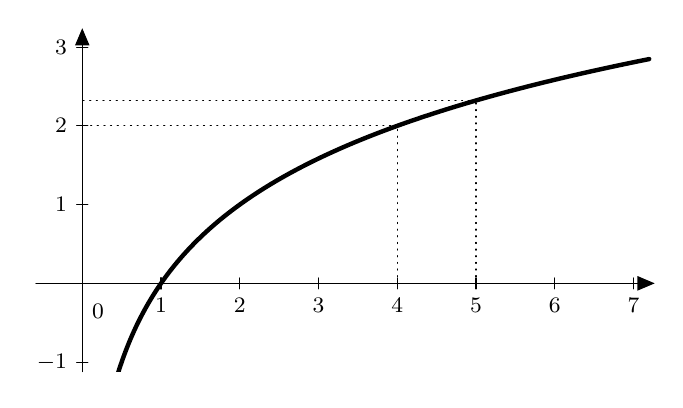
\begin{tikzpicture}[line cap=round,line join=round,>=triangle 45,x=1.0cm,y=1.0cm]
\draw[->,color=black] (-0.59,0) -- (7.27,0);
\foreach \x in {,1,2,3,4,5,6,7}
\draw[shift={(\x,0)},color=black] (0pt,2pt) -- (0pt,-2pt) node[below] {\footnotesize $\x$};
\draw[->,color=black] (0,-1.12) -- (0,3.24);
\foreach \y in {-1,1,2,3}
\draw[shift={(0,\y)},color=black] (2pt,0pt) -- (-2pt,0pt) node[left] {\footnotesize $\y$};
\draw[color=black] (0pt,-10pt) node[right] {\footnotesize $0$};
\clip(-0.59,-1.12) rectangle (7.27,3.24);
\draw[line width=1.6pt, smooth,samples=100,domain=0.1:7.2] plot(\x,{ln((\x))/ln(2)});
\draw [dotted] (4,0)-- (4,2);
\draw [dotted] (5,0)-- (5,2.32);
\draw [dotted] (4,2)-- (0,2);
\draw [dotted] (5,2.32)-- (0,2.32);
\end{tikzpicture}
\end{center}

Stel $f(x)=\log_2(x)$ en neem een waarde $x=4$ dicht bij de waarde $5$ die we willen benaderen.

We berekenen
\begin{enumerate}
  \item $\Delta x = 5-4 = 1$
  \item $\Delta y = \log_2(5) - \log_2(4) = \log_2(5) - 2$
  \item $df(x)=d\log_2(x)=\dfrac{1}{x\ln 2} dx$
\end{enumerate}

We maken nu gebruik van het feit dat $\Delta x=dx$ en $\Delta y \approx dy$ met $dy=df(9)$
\begin{align*}
    &&      \Delta y &\approx df(4)\\
\LRA&& \log_2(5) - 2 &\approx \dfrac{1}{4\ln 2} \cdot 1\\        
\LRA&&     \log_2(5) &\approx 2 + \dfrac{1}{4\ln 2} \cdot 1\\        
\LRA&&     \log_2(5) &\approx 2 + \dfrac{1}{4\cdot 0.7}\\        
\LRA&&     \log_2(5) &\approx 2.36\\        
\end{align*}

De werkelijke waarde afgerond op 2 decimalen is $\log_2 5 = 2.32$. We hebben dus een fout van 4 honderdsten.

\end{theorie}

\begin{oefening}
Benader
\begin{multicols}{3}
\begin{enumerate}[(a)]
  \itemsep.5em
  \item $\displaystyle \sqrt[3]{9}$
  \item $\displaystyle \sqrt{24}$
  \item $\displaystyle e^{0.2}$
  \item $\displaystyle \sqrt{9.5}$
  % next are from https://www.math24.net/approximation-differentials/
  \item $\displaystyle \sqrt[3]{30}$
  \item $\displaystyle \sqrt{50}$
  \item $\displaystyle \sqrt[4]{0.025}$
  \item $\displaystyle 8.2^\frac{2}{3}$
\end{enumerate}
\end{multicols}
\end{oefening}

\begin{oefening} % bron http://info.math4all.nl/MathAdore/vb-bb43-ex2b.html
De luchtdruk $p$ (in hectopascal $\hPa$) hangt af van de hoogte $h$ in $\km$ boven het aardoppervlak. In een luchtballon is de luchtdruk gemakkelijk te meten en wordt daaruit de hoogte berekend met de formule:
$$h = -6.5 \log \frac{p}{p_0}$$
Hierin is $p_0$ de luchtdruk op zeeniveau. Neem aan dat $p_0 = 1000 \hPa$.
Bereken nu de hoogte en de snelheid waarmee $h(p)$ verandert als $p = 920 \hPa$ wordt gemeten. 
\end{oefening}

\pagebreak
\section{Bepaalde integraal}

\begin{theorie}

\subsection{Definitie}

We beschouwen een willekeurige functie $y=f(x)$, positief tussen $a$ en $b$, en berekenen de oppervlakte $S$ begrepen tussen
\begin{itemize}
  \item de $x$-as: $y=0$,
  \item de grafiek van $y=f(x)$,
  \item de verticale $x=a$,
  \item de verticale $x=b$.
\end{itemize}

\begin{center}
\definecolor{dcrutc}{rgb}{0.8627,0.0784,0.2353}
\definecolor{sqsqsq}{rgb}{0.1255,0.1255,0.1255}
\begin{tikzpicture}[scale=1.5,line cap=round,line join=round,>=triangle 45,x=1.0cm,y=1.0cm]
\draw[->,color=black] (-1.3618,0) -- (7.1769,0);
\draw[color=black] (6.9069,0.0675) node [anchor=south west] { x};
\draw[->,color=black] (0,-1.2111) -- (0,3.5477);
\draw[color=black] (0.0844,3.2102) node [anchor=west] { y};
\clip(-1.3618,-1.2111) rectangle (7.1769,3.5477);
\draw[color=sqsqsq,fill=sqsqsq,fill opacity=0.1] {[smooth,samples=50,domain=1.0:6.0] plot(\x,{sin((2*\x-3)*180/pi)-(\x-3)^2/10+2})} -- (6,0) {[smooth,samples=50,domain=6.0:1.0] -- plot(\x,{0})} -- (1,0.7585) -- cycle;
\draw[line width=1.6pt, smooth,samples=100,domain=0.5:6.5] plot(\x,{sin((2*(\x)-3)*180/pi)-((\x)-3)^2/10+2});
\fill [color=black] (1,0) circle (2.0pt);
\draw[color=black] (1,-0.2) node {a};
\fill [color=black] (6,0) circle (2.0pt);
\draw[color=black] (6,-0.2) node {b};
\draw[color=black] (1.4,2.4) node {$f$};
\draw[color=black] (3,1) node {$S$};
\end{tikzpicture}
\end{center}

\begin{itemize}
  \item Verdeel $[a,b]$ in $n$ gelijke deelintervallen, elk met lengte
  $$\Delta x=\dfrac{b-a}{n}$$
  We krijgen dus de $n$ gelijke deelintervallen
  $$[x_0, x_1],[x_1, x_2],\ldots,[x_{n-1}, x_{n}]$$
  \item Het $k$-de interval, namelijk $[x_{k-1},x_{k}]$, heeft een
  \begin{itemize}
    \item kleinste functiewaarde: $\min_k f$
    \item grootste functiewaarde: $\max_k f$
  \end{itemize}
  \item We berekenen voor alle intervallen samen de
  \begin{itemize}
    \item ondersom (som van de oppervlakten rechthoekjes onder de functie),
    \begin{align*}
      s_n &= \min\nolimits_1 f\cdot \Delta x + \min\nolimits_2 f\cdot \Delta x + \ldots + \min\nolimits_n f\cdot \Delta x\\
          &= \sum_{k=1}^n \min\nolimits_k f\cdot\Delta x
    \end{align*}
    \item bovensom (som van de oppervlakten rechthoekjes boven de functie),
    \begin{align*}
      S_n &= \max\nolimits_1 f\cdot \Delta x + \max\nolimits_2 f\cdot \Delta x + \ldots + \max\nolimits_n f\cdot \Delta x\\
          &= \sum_{k=1}^n \max\nolimits_k f\cdot\Delta x
    \end{align*}
  \end{itemize}
  \item De gevraagde oppervlakte $S$ ligt dan tussen deze 2 sommen:
  $$s_n \leq S \leq S_n$$
  \item Voor een oneindig aantal deelintervallen, $n\to+\infty$, krijgen we dus
  $$\lim_{n\to+\infty}s_n = \lim_{n\to+\infty}S_n = S$$
\end{itemize}

We noemen deze limiet $S$ de {\bf bepaalde integraal} van $f$ tussen de grenzen $a$ en $b$ en noteren
$$\int_a^b f(x)\;dx = \lim_{n\to+\infty}s_n = \lim_{n\to+\infty}S_n = S$$
met
\begin{itemize}
  \item $\displaystyle\int$ het {\bf integraalteken}
  \item $a$ de {\bf ondergrens} en $b$ de {\bf bovengrens}
  \item $f(x)$ het {\bf integrand} naar $x$
  \item $dx$ de {\bf differentiaal} naar $x$
\end{itemize}

Merk ook de elegantie van deze notatie op, de uitgetrokken $S$ staat voor sommatie, de differentiaal $dx$ staat voor een oneindig kleine $\Delta x$, bijvoorbeeld met de ondersommen:
$$\int_a^b f(x)\;dx = \lim_{n\to+\infty}\sum_{k=1}^n \min\nolimits_k f\cdot\Delta x$$

\pagebreak
\subsection{Voorbeeld}

Beschouw de functie
$$f(x)=x$$
en laten we het oppervlakte berekenen tussen $y=0$, $y=f(x)$, $x=0$, $x=1$.

\begin{center}
\definecolor{zzttqq}{rgb}{0.6,0.2,0}
\begin{tikzpicture}[scale=3.5,line cap=round,line join=round,>=triangle 45,x=1.0cm,y=1.0cm]
\draw[->,color=black] (-0.58,0) -- (1.76,0);
\foreach \x in {,1}
\draw[shift={(\x,0)},color=black] (0pt,2pt) -- (0pt,-2pt) node[below] {\footnotesize $\x$};
\draw[->,color=black] (0,-0.57) -- (0,1.33);
\foreach \y in {,1}
\draw[shift={(0,\y)},color=black] (2pt,0pt) -- (-2pt,0pt) node[left] {\footnotesize $\y$};
\draw[color=black] (0pt,-10pt) node[right] {\footnotesize $0$};
\clip(-0.58,-0.57) rectangle (1.76,1.33);
\draw[color=zzttqq,fill=zzttqq,fill opacity=0.1, smooth,samples=50,domain=0.0:1.0] plot(\x,{\x}) -- (1,0) -- (0,0) -- cycle;
\draw[line width=1.6pt, smooth,samples=100,domain=-0.5755180752138966:1.7618129400811133] plot(\x,{(\x)});
\draw (0,-0.57) -- (0,1.33);
\draw [dotted] (1,-0.57) -- (1,1.33);
\draw (0.63,0.97) node[anchor=north west] {f};
\end{tikzpicture}
\end{center}

\begin{itemize}
  \item We delen $[0,1]$ op in $n$ deelintervallen van lengte $\Delta x=\dfrac{1}{n}$:
  $$[0,\dfrac{1}{n}],\, [\dfrac{1}{n},\dfrac{2}{n}],\, [\dfrac{2}{n},\dfrac{3}{n}],\, \ldots,\, [\dfrac{n-2}{n},\dfrac{n-1}{n}],\, [\dfrac{n-1}{n},1]$$
  \item Op een deelinterval $[\dfrac{k-1}{n},\dfrac{k}{n}]$:
  \begin{itemize}
    \item kleinste waarde: $\min_k f = \dfrac{k-1}{n}$
    \item grootste waarde: $\max_k f = \dfrac{k}{n}$
  \end{itemize}
  \item Onder- en bovensom:
  \begin{itemize}
    \item ondersom: $s_n=\sum^n_{k=1}\min_k f \cdot \Delta x=\sum^n_{k=1}\dfrac{k-1}{n}\cdot\dfrac{1}{n}=\dfrac{n-1}{2n}$
    \item bovensom: $S_n=\sum^n_{k=1}\max_k f \cdot \Delta x=\sum^n_{k=1}\dfrac{k}{n}\cdot\dfrac{1}{n}=\dfrac{n+1}{2n}$
  \end{itemize}
  \item Limieten berekenen:
  $$\lim_{n\to+\infty}s_n=\lim_{n\to+\infty}\dfrac{n-1}{2n}=\dfrac{1}{2}$$
  $$\lim_{n\to+\infty}S_n=\lim_{n\to+\infty}\dfrac{n+1}{2n}=\dfrac{1}{2}$$
  \item Besluit:
  $$\int_0^1 x\;dx=\dfrac{1}{2}$$
\end{itemize}

\subsection{Eigenschappen}

\begin{itemize}
  \item Gelijke grenzen: $a=b \Rightarrow \mbox{opp}=0$
  $$\int_a^a f(x)\;dx = 0$$
  \item Wisselen van de grenzen: $a\leftrightarrow b \Rightarrow \Delta x \mbox{ verandert van teken}$
  $$\int_a^b f(x)\;dx = -\int_b^a f(x)\;dx$$
  \item Opsplitsen van de integraal: $\forall c\in[a,b]:$
  $$\int_a^b f(x)\;dx = \int_a^c f(x)\;dx + \int_c^b f(x)\;dx$$
  \item Lineariteit van de integraal: $\alpha, \beta\in\mathbb{R}$
  $$\int_a^b \alpha f(x) + \beta f(x)\;dx = \alpha \int_a^b f(x) \;dx+ \beta \int_a^b f(x)\;dx$$
\end{itemize}

\subsection{Primitieve functie}

We voeren een nieuwe notatie in
$$[F(x)]_a^b = F(b) - F(a)$$
en lezen dit als we berekenen $F$ van $a$ naar $b$.

\end{theorie}

\begin{oefening}
Bereken
\begin{multicols}{2}
\begin{enumerate}[(a)]
  \itemsep.5em
  \item $\displaystyle\left[2x-3\right]_1^3$ 
  \item $\displaystyle\left[x^2\right]_0^4$ 
  \item $\displaystyle\left[\ln x\right]_1^e$ 
  \item $\displaystyle\left[\ln x\right]_0^e$ 
\end{enumerate}
\end{multicols}
\end{oefening}

\begin{oefening}
\begin{enumerate}[(a)]
  \item Beschouw de functies
  $$f(x)=2 \mbox{ en } F(x)=2x$$
  \begin{itemize}
    \item Bereken de oppervlakte begrepen tussen $y=f(x),\;y=0,\;x=1,\;x=4$
    \item Bereken $[F(x)]_1^4$
    \item Wat is het verband tussen $f$ en $F$
  \end{itemize}
  \item Beschouw de functies
  $$f(x)=x \mbox{ en } F(x)=\dfrac{x^2}{2}$$
  \begin{itemize}
    \item Bereken de oppervlakte begrepen tussen $y=f(x),\;y=0,\;x=0,\;x=4$
    \item Bereken $[F(x)]_0^4$
    \item Wat is het verband tussen $f$ en $F$
  \end{itemize}
  \item Beschouw de functies
  $$f(x)=x \mbox{ en } F(x)=\dfrac{x^2}{2}$$
  \begin{itemize}
    \item Bereken de oppervlakte begrepen tussen $y=f(x),\;y=0,\;x=2,\;x=5$
    \item Bereken $[F(x)]_2^5$
    \item Wat is het verband tussen $f$ en $F$
  \end{itemize}
\end{enumerate}
\end{oefening}

\begin{theorie}

We krijgen volgende definitie:

T.o.v. een orthonormaal assenstelsel is de oppervlakte $S$ begrepen tussen $y=f(x),\;y=0,\;x=a,\;x=b$ gelijk aan
$$S=\left[F(x)\right]_a^b \mbox{ met } F'(x)=f(x)\;.$$ We noemen $F$ {\em een} {\bf primitieve functie} van $f$.

\end{theorie}

\begin{oefening}
Bepaal {\em alle} primitieve functies van
\begin{enumerate}[(a)]
  \item $f(x)=5$
  \item $f(x)=7$
  \item $f(x)=0$
  \item $f(x)=2x$
  \item $f(x)=x$
  \item $f(x)=3x^2$
  \item $f(x)=x^2$
  \item $f(x)=x^n$ met $n\in\mathbb{R}\setminus\{-1\}$
\end{enumerate}
\end{oefening}

\begin{theorie}

Merk op dat elke functie $f$ oneindig veel primitieve functies $F$ heeft.

\subsection{Een bepaalde integraal berekenen}

\paragraph{Stelling}

Is $f$ continu in $[a,b]$ en is $F$ een primitieve functie van $f$ in $[a,b]$ dan geldt
$$\int_a^b f(x)\;dx = [F(x)]_a^b$$

\paragraph*{Gevolg}
$$\int_a^b x^n\;dx = \left[\dfrac{x^{n+1}}{n+1}\right]_a^b \mbox{ met } n\in\mathbb{R}\setminus\{-1\}$$

\end{theorie}

\begin{oefening}
Bereken
\begin{multicols}{3}
\begin{enumerate}[(a)]
  \itemsep1em
  \item $\displaystyle \int_0^2 x^3 \;dx$
  \item $\displaystyle \int_{-1}^{1} x^2 \;dx$
  \item $\displaystyle \int_1^3 x^4 \;dx$
  \item $\displaystyle \int_{-4}^4 \;dx$
  \item $\displaystyle \int_{-1}^{1} x \;dx$
  \item $\displaystyle \int_{-1}^{1} |x| \;dx$
\end{enumerate}
\end{multicols}
\end{oefening}

\begin{theorie}

\paragraph*{Integraal van een veeltermfunctie}
M.b.v. de lineariteit van een bepaalde integraal kunnen we de bepaalde integraal van een veeltermfunctie berekenen, bijvoorbeeld
\begin{align*}
  \int_1^3 2x^3-3x+1 \;dx &= \int_1^3 2x^3 \;dx + \int_1^3 -3x \;dx + \int_1^3 1 \;dx\\
                          &= 2\int_1^3 x^3 \;dx - 3\int_1^3 x \;dx + \int_1^3 \;dx\\
                          &= 2\cdot\left[\dfrac{x^4}{4}\right]_1^3 - 3\cdot\left[\dfrac{x^2}{2}\right]_1^3 +2\cdot\left[x\right]_1^3\\
                          &= 2\cdot \left(\dfrac{81}{4}-\dfrac{1}{4}\right) - 3\cdot \left(\dfrac{9}{2}-\dfrac{1}{2}\right) + 2\cdot \left(3-1\right)\\
                          &= 40 - 12 + 2\\
                          &= 30
\end{align*}
of veel korter!
\begin{align*}
  \int_1^3 2x^3-3x+1 \;dx &= \cdot\left[2\cdot\dfrac{x^4}{4} - 3\cdot\dfrac{x^2}{2} +2\cdot x\right]_1^3\\
                          &= (2\cdot \dfrac{81}{4} - 3\cdot \dfrac{9}{2} + 2\cdot 3) - (2\cdot \dfrac{1}{4} - 3\cdot \dfrac{1}{2} + 2\cdot 1)\\
                          &= 30
\end{align*}


\end{theorie}

\begin{oefening}
Bereken volgende bepaalde integralen
\begin{multicols}{2}
\begin{enumerate}[(a)]
\itemsep1em
  \item $\displaystyle \int_{-1}^2 (3x^2+2x-1)\;dx$
  \item $\displaystyle \int_{-4}^3 (6x^8+12x^5-\dfrac{1}{2}x^2)\;dx$
  \item $\displaystyle \int_{0}^5 (3x+5)^2\;dx$
  \item $\displaystyle \int_1^2 \dfrac{1}{x^2}\;dx$
  \item $\displaystyle \int_{-3}^{-1} \dfrac{4}{3x^3} \;dx$
  \item $\displaystyle \int_4^{16} \sqrt{x} \;dx$
  \item $\displaystyle \int_8^{27} \sqrt[3]{x} \;dx$
  \item $\displaystyle \int_2^8 \sqrt{2x} \;dx$
  \item $\displaystyle \int_8^{27} \dfrac{1}{\sqrt[3]{x}} \;dx$
  \item $\displaystyle \int_3^{16/3} \dfrac{x}{\sqrt{3x}} \;dx$
  \item $\displaystyle \int_{0}^3 (x+1)^3\;dx$
  \item $\displaystyle \int_{0}^2 (x+2)^6\;dx$
  \item $\displaystyle \int_{-1}^3 \dfrac{x+1}{x}\;dx$
  \item $\displaystyle \int_{-4}^4 \dfrac{x^2+2x+2}{4x^2}\;dx$
  \item $\displaystyle \int_{4}^0 \sqrt{x}(x-2)\;dx$
\end{enumerate}
\end{multicols}
\end{oefening}

\begin{oefening}
Bereken
\begin{multicols}{2}
\begin{enumerate}[(a)]
\itemsep1em
  \item $\displaystyle \int_1^2 y^2+y^{-2} \;dy$
  \item $\displaystyle \int_{-1}^2 y^2+y^{-2} \;dy$
  \item $\displaystyle \int_1^2 \dfrac{2\omega^5 - \omega + 3}{\omega^2} \;d\omega$
  \item $\displaystyle \int_{25}^{-10} \;dR$
\end{enumerate}
\end{multicols}
\end{oefening}

\begin{oefening} % source http://tutorial.math.lamar.edu/Classes/CalcI/ComputingDefiniteIntegrals.aspx
Gegeven
$$f(x)=\begin{cases}6 & \mbox{ if } x > 1\\3x^2 & \mbox{ if } x \leq 1\\\end{cases}$$
Bepaal
$$\displaystyle \int_{10}^{22} f(x) \;dx \qquad\mbox{ en }\qquad \displaystyle \int_{-2}^{3} f(x) \;dx$$
\end{oefening}

\pagebreak
\section{Oppervlakteberekeningen}

\begin{theorie}

\subsection{Verband bepaalde integraal en oppervlakte}

We houden rekening met 4 gevallen om de oppervlakte van een functie $f$ in een interval $[a,b]$ te berekenen m.b.v. een integraal:
\begin{itemize}
  \item $a<b$ en $f(x)\geq0$ in $[a,b]$
  \begin{align*}
    \int_a^b f(x)\; dx \geq 0 &\Rightarrow S=\int_a^b f(x)\; dx
  \end{align*}
  \item $a<b$ en $f(x)\leq0$ in $[a,b]$
  \begin{align*}
    \int_a^b f(x)\; dx \leq 0 &\Rightarrow S=-\int_a^b f(x)\; dx\\
                              &\Rightarrow S=|\int_a^b f(x)\; dx|\\
  \end{align*}
  \item $a>b$ en $f(x)\geq0$ in $[a,b]$
  \begin{align*}
    \int_a^b f(x)\; dx \leq 0 &\Rightarrow S=-\int_a^b f(x)\; dx\\
                              &\Rightarrow S=|\int_a^b f(x)\; dx|\\
  \end{align*}
  \item $a>b$ en $f(x)\leq0$ in $[a,b]$
  \begin{align*}
    \int_a^b f(x)\; dx \geq 0 &\Rightarrow S=-\int_a^b f(x)\; dx
  \end{align*}
\end{itemize}

\end{theorie}

\begin{oefening}
Bepaal de oppervlakte tussen
\begin{enumerate}[(a)]
\itemsep1em
  \item $\displaystyle y=x^2,\quad y=0,\quad x=0, \quad x=2$
  \item $\displaystyle y=x^2-6x,\quad y=0,\quad x=2, \quad x=4$
  \item $\displaystyle y=\sqrt{x},\quad y=0,\quad x=0, \quad x=9$
  \item $\displaystyle y=\sqrt[3]{x},\quad y=0,\quad x=0, \quad x=8$
  \item $\displaystyle y=\dfrac{x-1}{x},\quad y=0,\quad x=-3, \quad x=-1$
  \item $\displaystyle y=\dfrac{x^2-4}{x^2},\quad y=0,\quad x=1, \quad x=6$
\end{enumerate}
\end{oefening}

\begin{oefening}
Bepaal de oppervlakte tussen
\begin{enumerate}[(a)]
\itemsep1em
  \item $\displaystyle y=x(x-3),\quad y=0,\quad x=0, \quad x=5$
  \item $\displaystyle y=\sqrt{x},\quad y=\sqrt{x+1},\quad x=0, \quad x=4$
\end{enumerate}
\end{oefening}


\begin{oefening}
Bepaal de oppervlakte tussen de gegeven kromme en de $x$-as
\begin{multicols}{2}
\begin{enumerate}[(a)]
\itemsep1em
  \item $\displaystyle y=4x-x^2$
  \item $\displaystyle y=4x-x^3$
  \item $\displaystyle y=-x^3+5x^2-7x+3$
  \item $\displaystyle y=4x^4-8x^3-12x^2+16x+16$
\end{enumerate}
\end{multicols}
\end{oefening}

\begin{oefening}
Bepaal de oppervlakte tussen $f$ en $g$
\begin{enumerate}[(a)]
\itemsep1em
  \item $f(x)=x^2$ en $g(x)=2x$
  \item $f(x)=x$ en $g(x)=2x-x^2$
\end{enumerate}
\end{oefening}

\begin{oefening}
Bepaal de oppervlakte tussen
\begin{enumerate}[(a)]
\itemsep1em
  \item $x=y^3-26y+10$ en $x=40-6y^2-y^3$
  \item $x=|y|$ en $x=1-|y|$
  \item $y=|x|$ en $y=x^2-6$
  \item $y=\sqrt{x}$ en $y=x^2$
\end{enumerate}
\end{oefening}

\pagebreak
\section{Onbepaalde integraal}

\begin{oefening} {\scriptsize \em IJkingsproef industrieel ingenieur}\\
Bereken
$$\int \dfrac{(1+x)^2}{\sqrt{x}}\;dx$$
\begin{enumerate}[(A)]
\itemsep.5em
  \item $x^{5/2}+x^{3/2}+x^{1/2} + C$
  \item $\dfrac{(x+1)^3}{3\sqrt{x}} + C$
  \item $\dfrac{2}{5}x^{5/2}+\dfrac{2}{3}x^{3/2}+2x^{1/2} + C$
  \item $\dfrac{2}{5}x^{5/2}+\dfrac{4}{3}x^{3/2}+2x^{1/2} + C$
\end{enumerate}
\end{oefening}

\pagebreak
\section{Integratiemethoden}

\todo{Dit staat nog niet juist}

\begin{oefening}{\scriptsize Bron: Examencommissie Toelatingsexamen Arts en Tandarts, Juli 2016, id: 12190}\\
De afgeleide van een functie $f$, gedefinieerd op $]0,+\infty[$, is gegeven door $f'(x)=\ln x$. Bovendien is $f(e)=e^2$. Dan is $f(e^2)$ gelijk aan \hfill(geen giscorrectie)
\begin{enumerate}[(A)]
  \itemsep.5em
  \item $e^2$
  \item $2e^2$
  \item $2+e^2$
  \item $e^4$
\end{enumerate}
\end{oefening}

\pagebreak
\section{Toepassingen op integralen}


%\newpage
\end{document}
